% =======================================================
% STATISTICAL PHYSICS — LAB 1: Microstates of a System of Coins
% Section 1, Group B. Section structure follows the course template
% (Lab_1_Repot.pdf); layout and style follow E. Cortés's report style guide.
% Figures: report/figures/*.pdf, regenerated by `python main.py`.
% Compile from report/:  latexmk -pdf main.tex   (or pdflatex twice)
% =======================================================
\documentclass[11pt,a4paper]{article}

% ---------- PACKAGES ----------
\usepackage[utf8]{inputenc}
\usepackage[T1]{fontenc}
\usepackage[british]{babel}
\usepackage{geometry}
\geometry{a4paper, margin=2.1cm}
\usepackage{graphicx}
\graphicspath{{./}{figures/}}
\usepackage{amsmath, amssymb}
\usepackage{siunitx}
\sisetup{separate-uncertainty = true, multi-part-units = single, exponent-product = \times}
\usepackage{booktabs}
\usepackage{xcolor}
\usepackage{listings}
\usepackage{float}
\usepackage{caption}
\captionsetup{font=small, labelfont=bf}
\usepackage{subcaption}
\usepackage{fancyhdr}
\usepackage{setspace}
\setstretch{1.0}
\usepackage{hyperref}            % load last
\hypersetup{colorlinks=true, linkcolor=black, citecolor=black, urlcolor=blue}

% =======================================================
% REPORT DETAILS
% =======================================================
\newcommand{\labsubject}{Statistical Physics}
\newcommand{\reporttitle}{Microstates and Macroscopic Thermodynamics of a Binary System}
\newcommand{\shorttitle}{Lab 1: Microstates of a System of Coins}
\newcommand{\course}{Statistical Physics}
\newcommand{\instructor}{Prof. Víctor Tribaldos and Prof. Fernando J. Gómez Ruiz}
\newcommand{\reportdate}{November 4, 2026}
\newcommand{\repourl}{https://github.com/malenavilped-droid/Lab1_stats}
% Red marker for data still to be filled in. Remove every \fillin before submitting.
\newcommand{\fillin}[1]{\textcolor{red}{#1}}
% =======================================================

\newcommand{\authorrow}[3]{#1 & #2 & \texttt{@#3}\\}

% ---------- HEADER & FOOTER ----------
\pagestyle{fancy}
\fancyhf{}
\fancyhead[L]{Laboratory of \labsubject}
\fancyhead[R]{\shorttitle}
\fancyfoot[C]{\thepage}
\setlength{\headheight}{14pt}

% ---------- CODE SETTINGS ----------
\definecolor{codegray}{rgb}{0.5,0.5,0.5}
\definecolor{codepurple}{rgb}{0.58,0,0.82}
\definecolor{backcolour}{rgb}{0.95,0.95,0.92}
\lstdefinestyle{mystyle}{
    language=Python,
    backgroundcolor=\color{backcolour},
    commentstyle=\color{gray},
    keywordstyle=\color{blue},
    numberstyle=\tiny\color{codegray},
    stringstyle=\color{codepurple},
    basicstyle=\ttfamily\footnotesize,
    breaklines=true,
    captionpos=b,
    numbers=left,
    numbersep=5pt,
    showstringspaces=false
}
\lstset{style=mystyle}

\begin{document}

% ---------- TITLE PAGE ----------
\hypersetup{pageanchor=false}
\begin{titlepage}
  \centering
  {\LARGE Laboratory of \labsubject\par}
  \vspace{0.4cm}
  {\Large\bfseries \reporttitle\par}
  \vspace{0.3cm}
  {\large Laboratory Practice 1: Microstates of a System of Coins\par}
  \vspace{0.3cm}
  {\large\itshape Dual Bachelor in Engineering Physics and Industrial Technologies Engineering\par}
  \vspace{1.2cm}
  {\large\bfseries Section 1, Group B\par}
  \vspace{0.4cm}
  \begin{tabular}{lll}
    \toprule
    \textbf{Name} & \textbf{NIA} & \textbf{GitHub} \\
    \midrule
    \authorrow{Enrique Cortés Tirado}{100553551}{quiquecortestirado-afk}
    \authorrow{Malena Vílchez Pedrera}{100525717}{malenavilped-droid}
    \authorrow{Andrés Martín Muñoz}{100523003}{andrespepsi}
    \authorrow{Pablo Aguado González}{100524827}{PABLOSKYAGU}
    \bottomrule
  \end{tabular}\\[0.8cm]
  \textbf{Repository:} \url{\repourl} (release \texttt{v1.0})\\[0.4cm]
  \textbf{Course:} \course\\[0.3cm]
  \textbf{Instructors:} \instructor\\[0.3cm]
  \textbf{Date:} \reportdate
  \vfill
  
\includegraphics[width=0.3\textwidth]{uc3m_logo.png}
  \vfill
  {\large Department of Physics\\
   Universidad Carlos III de Madrid\par}
\end{titlepage}
\hypersetup{pageanchor=true}

% =======================================================
\section*{Abstract}
% =======================================================
This report studies a system of $N$ unbiased coins as an exact model of a two-state
assembly. A modular Python package, developed collaboratively on GitHub, enumerates the $2^N$
microstates bitwise and computes the multiplicities $\Omega(N,k)$ both exactly and in
log-space. Full enumeration was reached up to $N_{\max}=36$ coins in under \SI{5}{min}
($\SI{194.7}{s}$ for $6.9\times10^{10}$ microstates), with a run time that doubles with every
added coin. For the team parameter $N=109$, the most probable macrostate has
$P_{54}=0.0759$, the window $N/2\pm10$ already holds $95.5\,\%$ of the probability, and
obtaining only 8 heads would take on average $1.7\times10^{21}\,$s, about $3900$ times the age of
the universe. Stirling's approximation shows that the relative width of the distribution
scales as $1/\sqrt N\approx 3\times10^{-12}$ for $N\sim10^{23}$, which accounts for the
statistical character of the Second Law of Thermodynamics.

% =======================================================
\section{Introduction and Objectives}
\label{sec:intro}
% =======================================================
Many physical systems are built from constituents restricted to two discrete states: spin-$\tfrac12$
magnetic moments in a paramagnet, two-level atoms, or occupied and empty sites of a lattice gas.
A set of $N$ unbiased coins is the simplest representative of this class and can be solved
exactly, which makes it an ideal test bed for the foundations of statistical
mechanics~\cite{guide,schroeder}.

A \emph{microstate} is the full specification of every coin (e.g.\ \texttt{HHTHT}), so there are
$2^N$ of them, all equally probable. A \emph{macrostate} is defined only by the number of heads
$k$, irrespective of their order. Its multiplicity is the binomial coefficient
\begin{equation}
  \Omega(N,k)=\binom{N}{k}=\frac{N!}{k!\,(N-k)!},
  \qquad \sum_{k=0}^{N}\Omega(N,k)=2^N ,
  \label{eq:omega}
\end{equation}
and the probability of macrostate $k$ is
\begin{equation}
  P_k=\frac{\Omega(N,k)}{2^N}.
  \label{eq:pk}
\end{equation}
The link with thermodynamics is Boltzmann's entropy, $S=k_B\ln\Omega$, so that the entropy
difference between two macrostates is
\begin{equation}
  \frac{\Delta S_{k_1k_2}}{k_B}\equiv\frac{S(k_1)-S(k_2)}{k_B}
  =\ln\Omega(N,k_1)-\ln\Omega(N,k_2)=\ln\frac{P_{k_1}}{P_{k_2}} .
  \label{eq:ds}
\end{equation}
The last equality, which follows from Eq.~\eqref{eq:pk}, will be used repeatedly: an entropy
difference is the logarithm of a probability ratio.

In this report, the objective is to (i) enumerate the microstates of $N$ coins and determine
the computational limits of full enumeration and of the distribution $\Omega(N,k)$ (Part~1),
(ii) compute probabilities, entropy changes and waiting times for $N=100+M=109$ coins
(Part~2), and (iii) extrapolate every result to the thermodynamic limit $N\sim10^{23}$.

% =======================================================
\section{Methodology and Collaborative Workflow}
\label{sec:methods}
% =======================================================
\subsection{Environment and reproducibility}
All code runs in the Conda environment \texttt{statphys\_lab1} (Python 3.11, NumPy, SciPy,
Matplotlib, pytest), fully specified in \texttt{environment.yml}. A single command,
\texttt{python main.py}, regenerates every table and every figure of this report (vector PDF,
in \texttt{report/figures/}), and \texttt{pytest} runs the 105 unit tests.

\subsection{Version control and repository architecture}
Development followed a feature-branch workflow on GitHub: each module was written on its own
branch, opened as a pull request (PR) and merged into \texttt{main} only after another member
had reviewed it. Table~\ref{tab:repo} lists the modules, their owners and their PRs. Every use
of AI tools is logged in \texttt{AI\_STATEMENT.md} (Appendix~\ref{app:ai}).

\begin{table}[H]
  \centering
  \small
  \begin{tabular}{llll}
    \toprule
    Module & Content & Questions & Owner / PR (reviewer) \\
    \midrule
    \texttt{src/microstates.py} & bitwise enumeration, benchmark & 1a, 1b & Malena / \#4 (Pablo)\\
    \texttt{src/combinatorics.py} & exact and log-space $\Omega(N,k)$ & 1c, 1d & Pablo / \#5 (Andrés)\\
    \texttt{src/thermodynamics.py} & $P_k$, $\Delta S$, waiting times & 2a--2i, 2k & Andrés / \#6 (Enrique)\\
    \texttt{report/main.tex} & report, theory & 1e, 2j, 2k & Enrique / \#7(Malena)\\
    \texttt{tests/} & 105 pytest unit tests & all & each module's owner \\
    \bottomrule
  \end{tabular}
  \caption{Repository layout. Each module was developed on a feature branch and merged through a
  reviewed pull request.}
  \label{tab:repo}
\end{table}

\subsection{Numerical methods}
\label{sec:numerics}
\paragraph{Bitwise enumeration.} Each microstate is encoded as an integer
$s\in[0,2^N)$ whose bit $i$ is coin $i$ (1 = heads), so the number of heads is the
\emph{popcount} of $s$. Listing~\ref{lst:enum} shows the core of the enumeration: states are
visited in chunks of $2^{16}$ consecutive integers, the popcounts of a chunk are computed at once,
and \texttt{np.bincount} adds them to the histogram $\Omega(N,k)$.

\begin{lstlisting}[caption={Chunked bitwise enumeration (\texttt{src/microstates.py}).}, label={lst:enum}]
def macrostate_histogram_fast(n: int, chunk_bits: int = 16) -> list[int]:
    ...
    total = 1 << n                       # 2^n microstates
    chunk = 1 << min(chunk_bits, n)      # 2^16 states per chunk
    omega = np.zeros(n + 1, dtype=np.int64)
    for start in range(0, total, chunk):
        states = np.arange(start, start + chunk, dtype=np.uint64)
        omega += np.bincount(_popcount(states, n), minlength=n + 1)
    return [int(x) for x in omega]
\end{lstlisting}
Every state is still visited, but only one chunk is held in memory at a time
(about \SI{17}{B} per state, i.e.\ \SI{1.06}{MiB} in total, independently of $N$). The chunk
size was chosen so that it fits in the CPU's L2 cache: at $N=28$, chunks of $2^{16}$ ran about
twice as fast as chunks of $2^{22}$.

\paragraph{Exact and log-space multiplicities.} Exact values of $\Omega(N,k)$ are computed with
Python integers, which have arbitrary precision, using the multiplicative recurrence
\begin{equation*}
  \Omega(N,i)=\Omega(N,i-1)\,\frac{N+1-i}{i},
\end{equation*}
every step of which is an exact integer division.
For large $N$, everything is computed from the logarithm
\begin{equation}
  \ln\Omega(N,k)=\ln\Gamma(N+1)-\ln\Gamma(k+1)-\ln\Gamma(N-k+1),
  \label{eq:lgamma}
\end{equation}
which never overflows. Probabilities are obtained as $P_k=\exp(\ln\Omega-N\ln2)\le 1$, and
sums of probabilities with the log-sum-exp identity
$\ln\sum_k e^{x_k}=x_{\max}+\ln\sum_k e^{x_k-x_{\max}}$, which keeps every exponential
below one.

\paragraph{Validation.} The unit tests check the bitwise histogram against Eq.~\eqref{eq:omega}
for every $N$ tested, the exact rows against \texttt{math.comb} up to $N=1000$, the log-space
values against the logarithm of the exact integers (relative error below $10^{-12}$), the row
sums $\sum_k\Omega=2^N$, the symmetry $\Omega(N,k)=\Omega(N,N-k)$ and Pascal's rule. All
105 tests pass.

% =======================================================
\section{Computational Analysis of Microstates}
\label{sec:part1}
% =======================================================
\textit{The multiplicities and probabilities in this section and in Section~\ref{sec:part2} are
exact (integer arithmetic, or log-space with a relative error below $10^{-12}$) and carry no
statistical uncertainty. Only the run times are measured quantities.}

\subsection{Enumeration for \texorpdfstring{$N=7$}{N = 7}}
For $N=7$ there are $2^7=128$ microstates. Table~\ref{tab:n7} gives the multiplicity of each
macrostate, obtained by enumeration and identical to Eq.~\eqref{eq:omega}. The complete list
of the 128 microstates, grouped by macrostate, is given in Appendix~\ref{app:n7}.

\begin{table}[H]
  \centering
  \small
  \begin{tabular}{cccc}
    \toprule
    Heads $k$ & Tails $7-k$ & Sample microstate & $\Omega(7,k)$ \\
    \midrule
    7 & 0 & \texttt{HHHHHHH} & 1 \\
    6 & 1 & \texttt{HHHHHHT} & 7 \\
    5 & 2 & \texttt{HHHHHTT} & 21 \\
    4 & 3 & \texttt{HHHHTTT} & 35 \\
    3 & 4 & \texttt{HHHTTTT} & 35 \\
    2 & 5 & \texttt{HHTTTTT} & 21 \\
    1 & 6 & \texttt{HTTTTTT} & 7 \\
    0 & 7 & \texttt{TTTTTTT} & 1 \\
    \midrule
    \multicolumn{3}{r}{Total} & 128 \\
    \bottomrule
  \end{tabular}
  \caption{Macrostate multiplicity $\Omega(7,k)$ for $N=7$ coins, obtained by full enumeration
  (exact counts).}
  \label{tab:n7}
\end{table}

\subsection{Maximum \texorpdfstring{$N$}{N} for full enumeration}
\label{sec:1b}
The largest $N$ whose $2^N$ microstates can all be visited within \SI{5}{min} of wall-clock time
was found by increasing $N$ one coin at a time until the next run would exceed the limit.
Table~\ref{tab:enum} gives the measured times on the fastest team laptop
.

\begin{table}[H]
  \centering
  \small
  \begin{tabular}{cS[table-format=1.2e2]S[table-format=3.1]S[table-format=1.2e1]}
    \toprule
    $N$ & {Microstates $2^N$} & {Time [\si{s}]} & {Rate [states/s]} \\
    \midrule
    34 & 1.72e10 & 48.5  & 3.54e8 \\
    35 & 3.44e10 & 97.2  & 3.53e8 \\
    36 & 6.87e10 & 194.7 & 3.53e8 \\
    37 & 1.37e11 & {$\approx 389$ (est.)} & {---} \\
    \bottomrule
  \end{tabular}
  \caption{Full-enumeration times near the \SI{5}{min} limit (single runs; $N=37$ is extrapolated
  by doubling). The constant rate shows that the cost per microstate does not depend on $N$.
  The extra memory, measured with \texttt{tracemalloc} for $N=16$--24, is \SI{1.06}{MiB} and does not
  depend on $N$ by construction.}
  \label{tab:enum}
\end{table}

\noindent The result is
\begin{equation}
  \boxed{N_{\max}=36}\qquad(\SI{194.7}{s}\text{ for }2^{36}\approx6.9\times10^{10}\text{ microstates}).
  \label{eq:nmax}
\end{equation}
An independent run of the same code (\texttt{notebooks/microstates.ipynb}) gave
\SIlist{61.1;122.9;245.2}{s} for $N=34$, 35 and 36, so the result $N_{\max}=36$ is reproducible.

\paragraph{Time limit.} Every additional coin doubles the number of microstates, so the run time
grows as $t\propto 2^N=e^{N\ln2}$. The measured times confirm it: from $N=34$ to 36 the
slope is $\ln(194.7/48.5)/2=0.695$, against the theoretical $\ln2=0.693$. Figure~\ref{fig:enum}
shows the benchmark at small $N$ (mean $\pm$ standard deviation of 3 repeats). There, the
fitted slope ($0.47$) is lower than $\ln 2$ because runs of a few milliseconds are dominated by
fixed overheads (Python calls, array allocation). For this reason the limit is taken from the
measured runs of Table~\ref{tab:enum}, not from the extrapolated fit. Since the rate per state is
fixed by the hardware, a faster machine or compiled code would only shift $N_{\max}$ by
$\log_2$ of the speed-up: a computer ten times faster would reach $N=39$.

\paragraph{Memory limit.} Storing every microstate would require $O(N\,2^N)$ bits: about
\SI{310}{GB} for $N=36$ (or \SI{550}{GB} as 64-bit integers), far beyond any laptop. The chunked
generator of Listing~\ref{lst:enum} makes the memory cost $O(1)$ in $N$ (\SI{1.06}{MiB}), so
time, not memory, is the limiting factor.

\begin{figure}[!htbp]
  \centering
  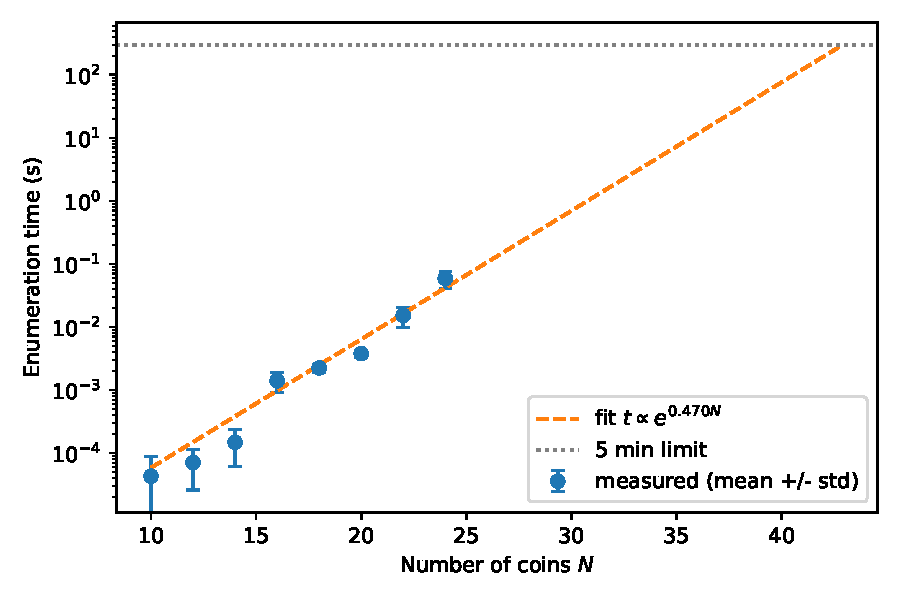
\includegraphics[width=0.55\textwidth]{enumeration_time.pdf}
  \caption{Full-enumeration time as a function of the number of coins $N$, on a logarithmic
  axis. Points are the mean $\pm$ standard deviation of 3 repeats (where not visible, the error
  bars are smaller than the marker); the dashed line is the least-squares fit of $\ln t$ against
  $N$, and the dotted line marks the \SI{5}{min} limit.}
  \label{fig:enum}
\end{figure}

\subsection{Macrostate distributions for \texorpdfstring{$N=20,50,80,100$}{N = 20, 50, 80, 100}}
Figure~\ref{fig:omega}(a) shows the exact multiplicities $\Omega(N,k)$ for the four values of $N$.
Every curve is symmetric about $k=N/2$, and its height grows as $2^N$: for $N=100$,
$\Omega(100,50)\approx1.0\times10^{29}$ out of $2^{100}\approx1.27\times10^{30}$ microstates.
Figure~\ref{fig:omega}(b) normalises the four curves as a density in $k/N$. Notably, the
peak becomes higher and narrower as $N$ grows: the larger the system, the more the fraction of
heads concentrates around $1/2$. This narrowing is quantified in Section~\ref{sec:limit}.

\begin{figure}[!htbp]
  \centering
  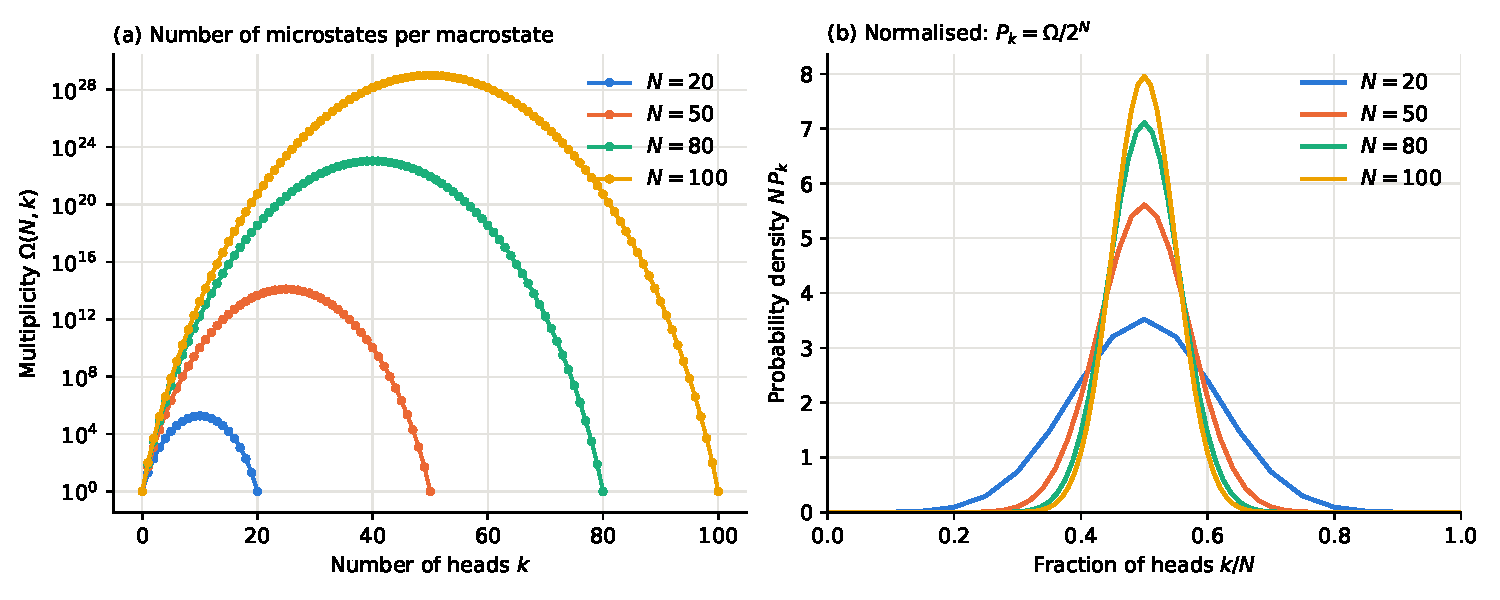
\includegraphics[width=0.92\textwidth]{multiplicity_distribution.pdf}
  \caption{(a) Exact multiplicity $\Omega(N,k)$ (dimensionless, logarithmic axis) against the
  number of heads $k$ for $N=20,50,80,100$. (b) The same distributions as the probability
  density $N P_k$ against the fraction of heads $k/N$; the area under each curve is 1. All
  values are exact.}
  \label{fig:omega}
\end{figure}

\subsection{Maximum \texorpdfstring{$N$}{N} for the distribution}
\label{sec:1d}
The largest $N$ for which $\Omega(N,k)$ can be computed and plotted depends on the method, as
summarised in Table~\ref{tab:limits}.

\begin{table}[H]
  \centering
  \small
  \begin{tabular}{lll}
    \toprule
    Method & Largest $N$ & Limiting factor \\
    \midrule
    float64 factorials $N!/(k!(N-k)!)$ & 170 & $171!>1.8\times10^{308}$ overflows \\
    float64 value of $\Omega(N,N/2)$ & 1029 & the peak itself overflows \\
    exact integers & no hard limit & cost grows as $\sim N^2$ \\
    log-space, Eq.~\eqref{eq:lgamma} & no overflow & precision, tail underflow, $N+1$ points \\
    \bottomrule
  \end{tabular}
  \caption{Practical limits for computing the full distribution $\Omega(N,k)$, $k=0,\dots,N$.}
  \label{tab:limits}
\end{table}

Naive floating-point factorials fail at $N=171$, and even the final value $\Omega(N,N/2)$ no
longer fits in a float64 beyond $N=1029$. Exact integers never overflow, but each row requires
$N/2$ multiplications of numbers with up to $N$ bits, so the cost grows roughly as $N^2$.
Log-space has no overflow at all; its limits are (i) precision, since $\ln\Omega\sim N\ln2$
and its rounding grows with $N$ ($|\sum_k P_k-1|$ grows from $3\times10^{-14}$ at $N=100$ to
$10^{-8}$ at $N=10^7$), (ii) underflow of the tails (at $N=10^4$ only 3799 of the 10001 values
$P_k$ are non-zero in float64), and (iii) memory and plotting of $N+1$ points. In practice,
plotting is meaningful up to $N\sim10^{6}$--$10^{7}$, where the peak is already narrower than
a pixel on a $k/N$ axis.

\subsection{Extrapolation to the thermodynamic limit \texorpdfstring{($N\sim10^{23}$)}{(N ~ 1e23)}}
\label{sec:limit}
For large $N$, Stirling's formula $\ln n!\approx n\ln n-n+\tfrac12\ln(2\pi n)$ turns the
binomial distribution into a Gaussian. Writing $k=N/2+x$ (Appendix~\ref{app:stirling}),
\begin{equation}
  \ln\Omega(N,k)\approx N\ln2-\frac12\ln\frac{\pi N}{2}-\frac{2x^2}{N}
  \quad\Longrightarrow\quad
  P_k\approx\sqrt{\frac{2}{\pi N}}\;\exp\!\left[-\frac{(k-N/2)^2}{2\sigma^2}\right],
  \qquad \sigma=\frac{\sqrt N}{2}.
  \label{eq:gauss}
\end{equation}
The mean is $\mu=N/2$, so the relative width of the peak is
\begin{equation}
  \frac{\sigma}{\mu}=\frac{1}{\sqrt N}\;\xrightarrow{\;N=10^{23}\;}\;3.2\times10^{-12}.
  \label{eq:width}
\end{equation}
For $N=10^{23}$ the absolute width $\sigma\approx1.6\times10^{11}$ coins is enormous, but the
fraction of heads $k/N$ is fixed to $1/2$ within a few parts in $10^{12}$, far below any
measurement resolution: the distribution in $k/N$ is effectively a Dirac delta. Physically, the
macrostate of maximum multiplicity is the only one ever observed, which is why a macroscopic
system has well-defined thermodynamic variables. At the same time, the height of the peak,
$P_{N/2}\approx\sqrt{2/(\pi N)}=2.5\times10^{-12}$, tends to zero: no \emph{single} value of $k$
is likely, only a narrow \emph{relative} window. The checks at $N=109$ confirm Eq.~\eqref{eq:gauss}:
$\sqrt{2/(\pi N)}=0.0764$ against the exact $P_{54}=0.0759$, and the Gaussian estimate of the
window $N/2\pm10$ is $0.9557$ against the exact $0.9552$.

% =======================================================
\section{Probabilities, Entropy and Thermodynamics}
\label{sec:part2}
% =======================================================
\subsection{Parameter assignment and conventions}
The last two digits of the members' NIAs are 03, 27, 17 and 51. Their harmonic mean is
\begin{equation}
  M=\frac{4}{\frac13+\frac1{27}+\frac1{17}+\frac1{51}}=8.9126,
  \label{eq:M}
\end{equation}
which rounded to the nearest integer gives $\boxed{M=9}$ and therefore $\boxed{N=109}$.
Two conventions follow from $N$ being odd:
\begin{itemize}
  \item $N/2=54.5$ is not a macrostate. We take $N/2\to\lfloor N/2\rfloor=54$. Since
  $\Omega(N,k)=\Omega(N,N-k)$, $P_{54}=P_{55}$ exactly, so the results of (b) and (g) do not
  depend on this choice. However, windows centred on 54 are not symmetric about the true centre
  54.5, which is why $P_{54}/P_{64}\neq P_{54}/P_{44}$ in (i).
  \item Question (d) is stated in tails: $54\pm20$ tails, i.e.\ 34--74 tails, corresponds to
  $35\le k\le75$ heads.
\end{itemize}
Entropy differences are given in units of $k_B$, the natural unit of Eq.~\eqref{eq:ds}; the
values in \si{J/K} (with $k_B=\SI{1.380649e-23}{J/K}$, exact in SI) follow by multiplication.

\subsection{Probability and entropy analysis}
Table~\ref{tab:part2} collects every result of questions (a)--(i), and Figure~\ref{fig:part2}
locates each macrostate on the distribution.

\begin{table}[H]
  \centering
  \small
  \begin{tabular}{clll}
    \toprule
    & Quantity & Macrostate(s) & Value \\
    \midrule
    (a) & $P_{30}$ & $k=30$ & $9.3747\times10^{-7}$ \\
    (b) & $P_{N/2}$ (most probable) & $k=54$ & $0.075903$ \\
    (c) & $\sum P_k$, $N/2\pm10$ heads & $44\le k\le64$ & $0.955238$ \\
    (d) & $\sum P_k$, $N/2\pm20$ tails & $35\le k\le75$ & $0.999923$ \\
    (e) & $\Delta S/k_B$ (high disorder $\to$ max.) & $k_1=79$, $k_2=54$ & $-11.302$ \quad($\SI{-1.560e-22}{J/K}$) \\
    (f) & $\Delta S/k_B$ (moderate $\to$ max.) & $k_1=64$, $k_2=54$ & $-1.645$ \quad($\SI{-2.271e-23}{J/K}$) \\
    (g) & $\Delta S/k_B$ (max.\ $\to$ high order) & $k_1=54$, $k_2=20$ & $+23.341$ \quad($\SI{+3.223e-22}{J/K}$) \\
    (h) & $\langle t\rangle$ for 8 heads & $k=8$ & $\SI{1.708e21}{s}=\SI{5.41e13}{yr}$ \\
    (i) & $P_{N/2}/P_{M+10}$ & $k=19$ & $6.166\times10^{10}$ \\
        & $P_{N/2}/P_{M-10}$ & $k=-1$ & $\infty$ (impossible macrostate) \\
        & $P_{N/2}/P_{N/2+10}$ & $k=64$ & $5.179$ \\
        & $P_{N/2}/P_{N/2-10}$ & $k=44$ & $7.481$ \\
    \bottomrule
  \end{tabular}
  \caption{Part 2 results for $N=109$ coins ($N/2\to54$). Probabilities and $\Delta S/k_B$ are
  dimensionless and exact (log-space, relative error $<10^{-12}$ against exact integers);
  $\langle t\rangle$ assumes one throw of the 109 coins per second.}
  \label{tab:part2}
\end{table}

\begin{figure}[!htbp]
  \centering
  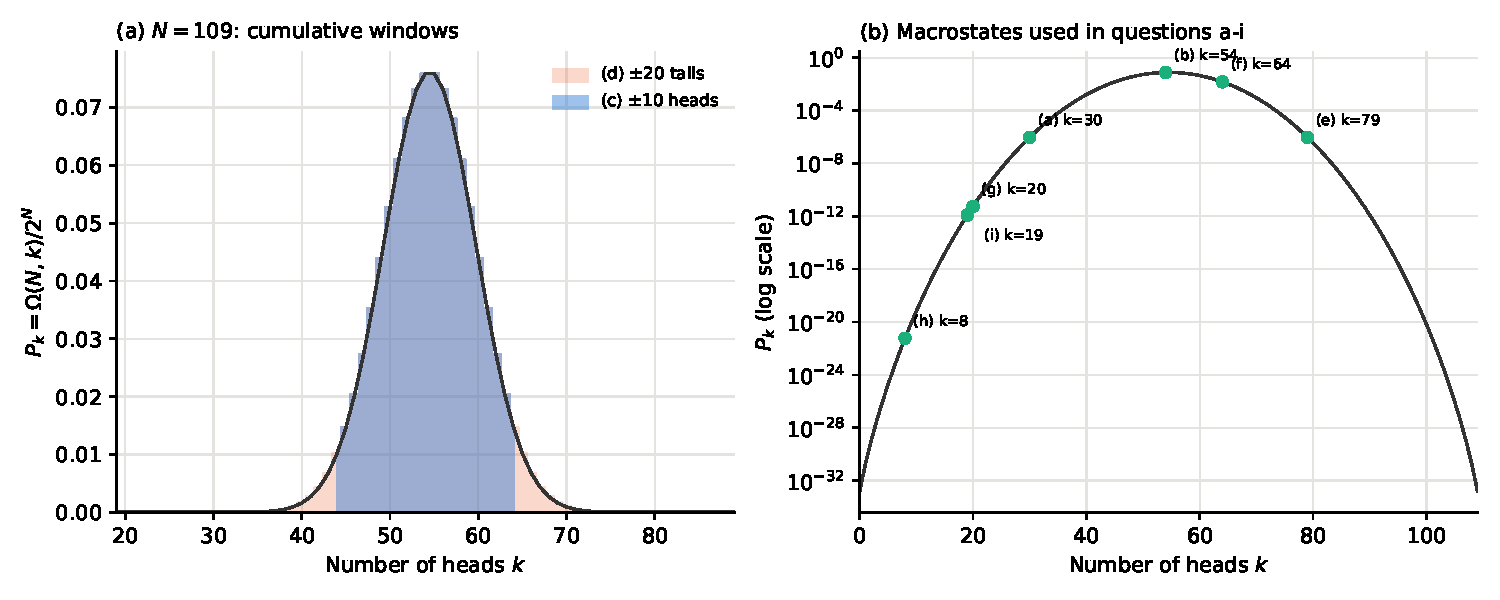
\includegraphics[width=0.92\textwidth]{part2_distribution.pdf}
  \caption{Probability distribution $P_k$ (dimensionless, exact) for $N=109$ coins. (a) Linear
  scale; the shaded areas are the windows of questions (c) ($44\le k\le64$, blue) and (d)
  ($35\le k\le75$, orange). (b) Logarithmic scale, with the macrostate used in each question
  (a)--(i) marked.}
  \label{fig:part2}
\end{figure}

\paragraph{Probabilities (a)--(d).} Even the most probable macrostate is observed only in
$7.6\,\%$ of the throws, whereas the window of $\pm10$ heads ($\approx\pm1.9\sigma$, with
$\sigma=\sqrt{109}/2=5.22$) already contains $95.5\,\%$ of the probability and the window of
$\pm20$ ($\approx\pm3.8\sigma$) contains all but $8\times10^{-5}$ of it. Thirty heads, only
$4.7\sigma$ from the centre, is already a one-in-a-million event.

\paragraph{Entropy (e)--(g).} By Eq.~\eqref{eq:ds}, $\Delta S/k_B$ is the logarithm of a
probability ratio. Moving away from the maximum lowers the entropy, so (e) and (f) are
negative, and the further the move, the larger the drop: $-1.6\,k_B$ for 10 heads away and
$-11.3\,k_B$ for 25 heads away, which is roughly quadratic in the displacement, as
Eq.~\eqref{eq:gauss} predicts ($-2x^2/N$ gives $-1.8$ and $-11.5$). Incidentally, $k=79$
has exactly the same probability as $k=30$ in (a), since $109-79=30$. Conversely, (g) is
positive: the maximally disordered macrostate has $e^{23.3}\approx1.4\times10^{10}$ times
more microstates than the ordered one with 20 heads. In \si{J/K} all these values are of order
$10^{-22}$, which shows why entropy differences of a few coins are thermodynamically invisible.

\paragraph{Waiting time (h).} Each throw of the $N$ coins is an independent trial that succeeds
with probability $p=P_8=5.85\times10^{-22}$. The number of throws until the first success is
therefore geometrically distributed with mean $1/p$, so at one throw per second
\begin{equation}
  \langle t\rangle=\frac{1}{P_8}\,\si{s}=\SI{1.708e21}{s}=\SI{5.41e13}{yr}
  \approx 3.9\times10^{3}\;t_{\text{universe}},
  \label{eq:wait}
\end{equation}
with $t_{\text{universe}}=\SI{13.787}{Gyr}=\SI{4.35e17}{s}$~\cite{planck}. The standard deviation
of a geometric distribution is $\sqrt{1-p}/p\approx\langle t\rangle$, so the waiting time is as
uncertain as it is long, but no realistic fluctuation makes it observable.

\paragraph{Likelihood ratio (i).} The guide asks for the ratio to a macrostate with ``$M\pm10$''
heads. Read literally, this gives $k=19$, for which the most probable state is
$6.2\times10^{10}$ times more likely, and $k=-1$, which has no microstates ($P=0$, infinite
ratio). Since the second value is meaningless, we also give the ratio for $N/2\pm10$, which is
likely the intended comparison: only $5.2$ and $7.5$. The difference between $P_{54}/P_{64}$ and
$P_{54}/P_{44}$ comes from the asymmetry of the convention $N/2\to54$. Note that a ratio of
individual probabilities $P_k$ is used, not of cumulative windows. As a cross-check,
$\ln(P_{54}/P_{64})=\ln5.179=1.645=-\Delta S$ of question (f).

\subsection{Second Law of Thermodynamics interpretation (j)}
\label{sec:2ndlaw}
None of these results contradicts the Second Law, but some of them, (e) and (f), describe
spontaneous decreases of entropy. If the coins are rethrown repeatedly, a system that is at
$k=54$ will sometimes be found at $k=64$ or $k=79$, with $\Delta S<0$. Indeed, for $N=109$ such
fluctuations are frequent: $P_{64}/P_{54}=e^{\Delta S/k_B}=0.19$.

The resolution is that the Second Law is a statistical statement. Every microstate is equally
probable and the underlying dynamics (here, each throw) has no preferred direction. The
macrostate $k=N/2$ dominates only because it contains overwhelmingly more microstates.
Equation~\eqref{eq:ds} gives the probability of a fluctuation that lowers the entropy by
$|\Delta S|$ directly:
\begin{equation}
  \frac{P_{\text{fluct}}}{P_{\text{eq}}}=e^{-|\Delta S|/k_B}.
  \label{eq:fluct}
\end{equation}
Decreases of a few $k_B$ are common and decreases of order $10\,k_B$ are rare but observable,
while a decrease to a highly ordered state is effectively never observed: Eq.~\eqref{eq:wait}
shows that even with only 109 coins, eight heads would take longer than the age of the universe
thousands of times over. For a macroscopic deviation of the fraction of heads,
$\delta=k/N-\tfrac12$, Eq.~\eqref{eq:gauss} gives $|\Delta S|/k_B\approx2\delta^2N$, so its
probability decays as $e^{-cN}$. The Second Law is therefore not violated but is valid
\emph{with overwhelming probability}, a probability that tends to certainty as $N\to\infty$.

\subsection{Large-\texorpdfstring{$N$}{N} limit (k)}
\label{sec:2k}
For $N\sim10^{23}$, Eq.~\eqref{eq:lgamma} cannot be evaluated directly in float64, since
$\ln\Gamma(N+1)\approx5\times10^{24}$ and the 16 significant digits of a double are lost when two
such terms are subtracted. The values of Table~\ref{tab:2k} were therefore obtained from the
Gaussian form, Eq.~\eqref{eq:gauss}, near the peak, and from the exact small-$k$ form
$\ln\Omega\approx\sum_{i<k}\ln(N-i)-\ln k!$ for $k\ll N$. The value of $M$ is kept at 9.

\begin{table}[H]
  \centering
  \small
  \begin{tabular}{clll}
    \toprule
    & Quantity & $N=109$ & $N=10^{23}$ \\
    \midrule
    (a) & $P_{30}$ & $9.37\times10^{-7}$ & $10^{-3.01\times10^{22}}$ \\
    (b) & $P_{N/2}\approx\sqrt{2/(\pi N)}$ & $0.0759$ & $2.5\times10^{-12}$ \\
    (c) & $\sum P_k$, $N/2\pm10$ & $0.955$ & $5.3\times10^{-11}$ \\
    (d) & $\sum P_k$, $N/2\pm20$ & $0.99992$ & $1.0\times10^{-10}$ \\
    (e) & $\Delta S/k_B\approx-2(25)^2/N$ & $-11.3$ & $-1.25\times10^{-20}$ \\
    (f) & $\Delta S/k_B\approx-2(10)^2/N$ & $-1.64$ & $-2.0\times10^{-21}$ \\
    (g) & $\Delta S/k_B\approx N\ln2$ & $+23.3$ & $+6.93\times10^{22}$ \\
    (h) & $\langle t\rangle=1/P_8$ [\si{s}] & $1.7\times10^{21}$ & $10^{3.01\times10^{22}}$ \\
    (i) & $P_{N/2}/P_{M+10}$ & $6.2\times10^{10}$ & $10^{3.01\times10^{22}}$ \\
        & $P_{N/2}/P_{N/2\pm10}\approx e^{200/N}$ & $5.2$, $7.5$ & $1+2\times10^{-21}$ \\
    \bottomrule
  \end{tabular}
  \caption{Part 2 for $N=109$ (exact) and for $N=10^{23}$ (Stirling/Gaussian limit, leading
  order). All quantities are dimensionless except $\langle t\rangle$.}
  \label{tab:2k}
\end{table}

Two scalings explain every entry. First, \emph{fixed} windows lose all their probability while
\emph{relative} windows gain it all. The windows of (c) and (d) are fixed at $\pm10$ and $\pm20$
coins, much narrower than $\sigma\approx1.6\times10^{11}$, so their probability tends to zero,
like $P_{N/2}$ itself. In contrast, a window of fixed relative width, e.g.\
$|k/N-\tfrac12|<10^{-10}$ (about $60\sigma$), contains essentially all the probability.
Second, \emph{fixed} displacements cost no entropy, while \emph{extensive} ones cost an
extensive amount. Moving 10 or 25 coins away from the maximum changes $S$ by $\sim-2x^2/N\to0$
in (e) and (f), and the ratios of (i) relative to $N/2\pm10$ tend to 1: such macrostates are
thermodynamically indistinguishable from equilibrium. However, any macrostate with a fixed number
of heads (30, 20, 8 or $M+10=19$) is an ordered state with $k/N\to0$. Its entropy deficit is
$\approx N\ln2\approx7\times10^{22}\,k_B$ (\SI{0.96}{J/K}), its probability is
$\approx2^{-N}$, and the waiting time of (h) becomes $10^{3\times10^{22}}$ seconds, a number
with no physical meaning. For (j), the conclusion of Section~\ref{sec:2ndlaw} becomes absolute:
fluctuations of a few coins still exist but are invisible ($\sigma/N\sim10^{-12}$), and
macroscopic decreases of entropy have probability $e^{-cN}$ with $N=10^{23}$. In the
thermodynamic limit, the statistical Second Law becomes indistinguishable from a strict law.

% =======================================================
\section{Conclusion}
\label{sec:conclusion}
% =======================================================
A system of $N$ coins was modelled with a tested, modular Python package developed through
reviewed pull requests. Full bitwise enumeration of the $2^N$ microstates was achieved up to
$N=36$ in \SI{194.7}{s}, a limit set by the exponential run time ($t\propto2^N$, measured slope
$0.695$ against $\ln2$), while a chunked generator kept the memory at \SI{1.06}{MiB}. Log-space
combinatorics removed every overflow, leaving precision and tail underflow as the only limits on
the distribution. For $N=109$, the probabilities and entropy changes show a sharply peaked
distribution in which ordered macrostates are extraordinarily improbable: eight heads would take
$1.7\times10^{21}\,$s to appear. Stirling's approximation turns the binomial into a Gaussian of
relative width $1/\sqrt N$, which for $N\sim10^{23}$ makes the equilibrium macrostate the only
observable one. Overall, the coin model reproduces the statistical foundation of the Second Law:
entropy decreases are not forbidden, only exponentially improbable in $N$.

% ---------- REFERENCES ----------
\begin{thebibliography}{9}
  \bibitem{guide} V. Tribaldos, \textit{Microstates of a System of Coins}, Statistical Physics,
  Laboratory Practice 1, Universidad Carlos III de Madrid, 2026.
  \bibitem{schroeder} D. V. Schroeder, \textit{An Introduction to Thermal Physics}, Addison-Wesley,
  2000, Ch.~2.
  \bibitem{planck} Planck Collaboration, ``Planck 2018 results. VI. Cosmological parameters'',
  \textit{Astron. Astrophys.} \textbf{641}, A6 (2020).
\end{thebibliography}

% =======================================================
\appendix
% =======================================================
\section{Microstates for \texorpdfstring{$N=7$}{N = 7}}
\label{app:n7}
The 128 microstates of $N=7$ coins (H = heads, T = tails), grouped by macrostate, as written by
\texttt{main.py} to \texttt{report/microstates\_N7.txt}.

{\footnotesize\ttfamily\raggedright
\textbf{7H 0T (1):} HHHHHHH\par\smallskip
\textbf{6H 1T (7):} HHHHHHT HHHHHTH HHHHTHH HHHTHHH HHTHHHH HTHHHHH THHHHHH\par\smallskip
\textbf{5H 2T (21):} HHHHHTT HHHHTHT HHHTHHT HHTHHHT HTHHHHT THHHHHT HHHHTTH HHHTHTH HHTHHTH
HTHHHTH THHHHTH HHHTTHH HHTHTHH HTHHTHH THHHTHH HHTTHHH HTHTHHH THHTHHH HTTHHHH THTHHHH
TTHHHHH\par\smallskip
\textbf{4H 3T (35):} HHHHTTT HHHTHTT HHTHHTT HTHHHTT THHHHTT HHHTTHT HHTHTHT HTHHTHT THHHTHT
HHTTHHT HTHTHHT THHTHHT HTTHHHT THTHHHT TTHHHHT HHHTTTH HHTHTTH HTHHTTH THHHTTH HHTTHTH
HTHTHTH THHTHTH HTTHHTH THTHHTH TTHHHTH HHTTTHH HTHTTHH THHTTHH HTTHTHH THTHTHH TTHHTHH
HTTTHHH THTTHHH TTHTHHH TTTHHHH\par\smallskip
\textbf{3H 4T (35):} HHHTTTT HHTHTTT HTHHTTT THHHTTT HHTTHTT HTHTHTT THHTHTT HTTHHTT THTHHTT
TTHHHTT HHTTTHT HTHTTHT THHTTHT HTTHTHT THTHTHT TTHHTHT HTTTHHT THTTHHT TTHTHHT TTTHHHT
HHTTTTH HTHTTTH THHTTTH HTTHTTH THTHTTH TTHHTTH HTTTHTH THTTHTH TTHTHTH TTTHHTH HTTTTHH
THTTTHH TTHTTHH TTTHTHH TTTTHHH\par\smallskip
\textbf{2H 5T (21):} HHTTTTT HTHTTTT THHTTTT HTTHTTT THTHTTT TTHHTTT HTTTHTT THTTHTT TTHTHTT TTTHHTT HTTTTHT THTTTHT TTHTTHT TTTHTHT TTTTHHT HTTTTTH THTTTTH TTHTTTH TTTHTTH TTTTHTH TTTTTHH\par\smallskip
\textbf{1H 6T (7):} HTTTTTT THTTTTT TTHTTTT TTTHTTT TTTTHTT TTTTTHT TTTTTTH\par\smallskip
\textbf{0H 7T (1):} TTTTTTT\par}

\section{Gaussian limit of the binomial distribution}
\label{app:stirling}
With Stirling's formula $\ln n!\approx n\ln n-n+\frac12\ln(2\pi n)$ and the notation
$k=\frac N2(1+\delta)$, $N-k=\frac N2(1-\delta)$, where $\delta=2x/N$ and $x=k-N/2$, the linear
terms $-n$ cancel and
\begin{align}
  \ln\Omega(N,k)&=\ln N!-\ln k!-\ln(N-k)! \nonumber\\
  &\approx -N\!\left[\tfrac{1+\delta}{2}\ln\tfrac{1+\delta}{2}
     +\tfrac{1-\delta}{2}\ln\tfrac{1-\delta}{2}\right]
     -\tfrac12\ln\!\left[\tfrac{\pi N}{2}(1-\delta^2)\right] \nonumber\\
  &= N\ln2-\tfrac N2\left[(1+\delta)\ln(1+\delta)+(1-\delta)\ln(1-\delta)\right]
     -\tfrac12\ln\tfrac{\pi N}{2}-\tfrac12\ln(1-\delta^2).
  \label{eq:app1}
\end{align}
Expanding for $|\delta|\ll1$, $(1+\delta)\ln(1+\delta)+(1-\delta)\ln(1-\delta)=\delta^2+\delta^4/6+\dots$
and $\ln(1-\delta^2)\approx-\delta^2$, so to leading order
\begin{equation}
  \ln\Omega(N,k)\approx N\ln2-\tfrac12\ln\tfrac{\pi N}{2}-\tfrac{N\delta^2}{2}
  =N\ln2-\tfrac12\ln\tfrac{\pi N}{2}-\tfrac{2x^2}{N},
  \label{eq:app2}
\end{equation}
which is Eq.~\eqref{eq:gauss}. Dividing by $2^N$ gives a normalised Gaussian with
$\sigma^2=N/4$, since $\sqrt{2/(\pi N)}=1/(\sigma\sqrt{2\pi})$. The neglected terms are of
relative order $x^4/N^3$, so the Gaussian is accurate within a few $\sigma$ of the peak. Far in
the tails ($k/N\to0$), Eq.~\eqref{eq:app1} must be used instead. Its bracket is minus the
binary entropy of the fraction $k/N$, so $P_k\approx e^{-N[\ln2-H(k/N)]}\to2^{-N}$ for
ordered states.

\section{AI Collaboration and Audit Statement}
\label{app:ai}
In accordance with the course project guidelines, AI tools (Claude) were used as code and
writing assistants. Every query, the output it produced, and what the team changed or verified
is logged in \texttt{AI\_STATEMENT.md} in the repository~(\url{\repourl}). All AI-generated code
is backed by unit tests (105 pytest tests), every numerical result in this report was
cross-checked against exact integer arithmetic, and every member reviewed the code to be able
to explain it.

\end{document}
